\documentclass[10pt,a4paper,twocolumn]{article}
\usepackage[utf8]{inputenc}
\usepackage[T1]{fontenc}
\usepackage[french]{babel}
\usepackage{lmodern}
\usepackage[a4paper,top=1.5cm,bottom=1.6cm,left=1.5cm,right=1.5cm,columnsep=0.55cm]{geometry}
\usepackage{graphicx,booktabs,amsmath,array,xcolor,tikz,caption,enumitem}
\usepackage[hidelinks]{hyperref}
\usetikzlibrary{positioning,arrows.meta}
\captionsetup{font=small,labelfont=bf,skip=2pt}
\setlist{nosep,leftmargin=*}
\setlength{\parskip}{0pt}
\setlength{\textfloatsep}{6pt plus 2pt minus 2pt}
\setlength{\floatsep}{5pt plus 2pt minus 2pt}
\setlength{\dbltextfloatsep}{6pt plus 2pt minus 2pt}
\renewcommand{\arraystretch}{1.04}
\newcolumntype{L}[1]{>{\raggedright\arraybackslash}p{#1}}
\definecolor{olive}{RGB}{62,96,44}
\definecolor{retro}{RGB}{176,96,20}
\newcommand{\retro}{\textcolor{retro}{\textsuperscript{\textsf{R}}}}
\makeatletter
\renewcommand\section{\@startsection{section}{1}{\z@}{-1.3ex plus -.3ex}{0.5ex}{\normalfont\large\bfseries\color{olive}}}
\renewcommand\subsection{\@startsection{subsection}{2}{\z@}{-1.0ex plus -.2ex}{0.3ex}{\normalfont\normalsize\bfseries}}
\makeatother
\raggedbottom

\begin{document}

\twocolumn[{%
\begin{center}
{\small OliveSmart OLV-6 --- 5IIR, Framework J2EE et Architecture Microservices --- Deep Learning --- 2026--2027}\\[0.15cm]
{\Large\bfseries\color{olive} Détection de la disparition apparente d'oliviers sur images satellitaires multi-dates :
comparaison de cinq méthodes sur un test spatial commun}\\[0.2cm]
{\normalsize NAZIH Salma \quad GARTITE Yassine \quad TECHA Abderrahmane}
\end{center}
\begin{small}
\noindent\textbf{Résumé ---} Nous comparons cinq méthodes pour repérer, sur des images WorldView-2 de 2019, 2020 et 2021 (jeu
OQDS), les oliviers dont la couronne \emph{disparaît} : seuil, CUSUM, Isolation Forest, réseau siamois convolutionnel (Siamese
CNN) et TCN. La cible est un \emph{proxy} de disparition apparente, non un diagnostic sanitaire. Après contrôle qualité,
71\,956 arbres sont répartis par blocs spatiaux de 250\,m (test : 10\,205 arbres, 2,32\,\% de positifs). Dans la comparaison
pré-spécifiée (phase~1, sélection sur validation, test ouvert une fois), le Siamese CNN obtient la meilleure PR-AUC (0,220) et
le meilleur F1 (0,322), mais ne retrouve que 82 des 237 positifs. Des analyses \emph{rétrospectives} (phase~2) montrent qu'il
était sous-entraîné : une version révisée (Siamese~v2, ensemble de 5 graines) atteint 0,486 de PR-AUC et 72\,\% de rappel sur
le test d'origine, mais $0{,}33\pm0{,}14$ en moyenne sur 15 partitions géographiques, quelle que soit la taille des blocs
(250\,m à 1\,km). Une ablation attribue le gain à la comparaison des deux dates ; le modèle reste sensible à l'éclairage. Il
s'agit d'un outil de priorisation des inspections, à valider sur une région nouvelle et sur le terrain.\\[0.05cm]
\textbf{Mots-clés ---} olivier ; télédétection ; détection de changement ; réseau siamois ; validation spatiale ; classes rares.
\end{small}
\vspace{0.25cm}
}]

% ============================ 1. INTRODUCTION =============================
\section{Introduction}
Le suivi sanitaire des oliveraies à grande échelle se heurte au coût des inspections. OliveSmart vise à signaler les arbres
dont l'apparence change entre deux acquisitions, pour orienter les visites. Trois niveaux doivent rester distincts : la
\emph{présence d'une couronne}, sa \emph{disparition apparente} entre deux dates, et l'\emph{état phytosanitaire} réel. Dans
OQDS~\cite{oqds}, un positif est un arbre présent en 2019 puis absent ensuite : notre cible relève du deuxième niveau. Un arbre
malade mais visible est négatif, un arbre retiré pour une autre cause est positif.

\textbf{Lacune.} Comparer un modèle qui voit des images à des méthodes qui ne voient que des statistiques confond l'effet de
l'algorithme et celui de l'information d'entrée ; nous l'isolons par une ablation (section~\ref{sec:abl}).
\textbf{Questions.} RQ1 : la comparaison visuelle de deux dates apporte-t-elle plus que des indicateurs agrégés ? RQ2 : quel
compromis entre rappel, fausses alertes et charge d'inspection ? RQ3 : les résultats dépendent-ils d'artefacts (pixels noirs,
éclairage) ? \textbf{Contributions.} (1) Un audit des données, de l'étiquette et de la dépendance spatiale ; (2) une
comparaison de cinq méthodes sur une population de test commune ; (3) la traduction des scores en charge d'inspection. Nous
ne revendiquons ni nouvelle architecture ni détection de maladie.

\textbf{Travaux connexes.} La cartographie d'oliviers~\cite{lin} localise des arbres existants ; la classification de maladies
foliaires~\cite{raouhi} utilise d'autres images ; la détection de changement siamoise~\cite{bromley,daudt} prédit des cartes
\emph{par pixel}, alors que nous produisons une étiquette \emph{par arbre}. CUSUM~\cite{page}, Isolation Forest~\cite{iforest} et
les TCN~\cite{bai} servent de références. Des observations voisines partagent sol et éclairage : la validation doit être
spatiale~\cite{roberts,valavi}, et la PR-AUC est préférable à l'accuracy pour des positifs rares~\cite{saito}. Ces scores ne
sont pas directement comparables aux nôtres : notre étude est une comparaison interne au corpus.

% ============================== 2. DONNÉES ================================
\section{Données}
\textbf{Sources.} OQDS est la seule source qui associe, pour chaque arbre, une position et trois acquisitions co-enregistrées
au même capteur (Table~\ref{tab:datasets}). Ses limites : étiquette indirecte, un seul secteur d'environ 35\,km$^2$, trois
dates, et des fichiers dits « NDVI » qui sont en réalité des \emph{rendus RGBA 8 bits} sans proche infrarouge calibré. Leurs
intensités sont des caractéristiques d'image, pas un indice de végétation physique.

\begin{table*}[t]
\centering\small
\caption{Les quatre sources étudiées.}
\label{tab:datasets}
\setlength{\tabcolsep}{4pt}
\begin{tabular}{@{}lL{2.7cm}L{3.8cm}L{3.4cm}L{1.6cm}L{2.5cm}@{}}
\toprule
Source & Taille & Imagerie / résolution & Annotation & Période & Usage \\
\midrule
OQDS~\cite{oqds} & 77\,086 arbres (71\,956 retenus) & WorldView-2 RGB + rendu « NDVI » 8 bits, 0,5\,m, $\approx$35\,km$^2$ & point par arbre ; disparition apparente & 2019--2021 & benchmark principal \\
NEON~\cite{neon} & 41\,738 couronnes ; 38 sites & polygones issus d'imagerie aéroportée & espèce, hauteur, statut & 2017--2024 & audit : pas de paire d'années par arbre \\
Hyperspectral~\cite{hyper} & 76 oliviers & cubes $50\times50$ px, 138 bandes & stress \emph{Verticillium} (6 cas possibles) & une campagne & exploratoire \\
CrownsDb~\cite{crowns} & 5\,844 images ; 33\,479 boîtes & RGB drone, $608\times405$ à $5\,472\times3\,648$ px & boîtes de couronnes & non datée & audit qualité \\
\bottomrule
\end{tabular}
\end{table*}

\textbf{Contrôle qualité.} Après suppression de 104 doublons, 5\,026 observations invalides sont \emph{exclues} (non
réétiquetées) : 4\,959 patches majoritairement noirs (dont 98 positifs), 59 à couverture alpha insuffisante et 8 hors raster.
Les exclus sont moins souvent positifs (1,95\,\% contre 2,88\,\% ; $\chi^2$, $p=1{,}5\cdot10^{-4}$) : le filtrage écarte
4,5\,\% des positifs, un biais de sélection modeste mais réel.

\textbf{Partition et déséquilibre.} Les arbres sont regroupés en blocs de 250\,m affectés à une seule partition
(StratifiedGroupKFold) : entraînement 51\,425 arbres (3,00\,\% de positifs, 258 blocs), validation 10\,326 (2,82\,\%, 53 blocs),
test 10\,205 (2,32\,\%, 52 blocs). Les positifs sont très concentrés : ceux du test se trouvent dans \textbf{5 blocs sur 52}. Des
blocs voisins peuvent être dans deux partitions : 12\,\% des arbres test sont à moins de 16\,m d'un arbre d'entraînement
(médiane 62\,m), ce que nous contrôlons en section~\ref{sec:leak}.

\textbf{Radiométrie.} Sur 20\,000 arbres négatifs, la luminance moyenne vaut 165 (2019), 176 (2020) et 168 (2021), et la part
de pixels sombres (indicateur d'ombre) passe de 2,3\,\% à 1,4\,\% puis 2,1\,\%. Par bloc, la variation 2019$\to$2021 va de $-6$
à $+10$ (déciles 10--90\,\%) : un arbre peut changer d'apparence sans disparaître. Les dates exactes n'étant pas fournies,
l'effet saison ne peut pas être séparé de l'effet capteur (Figure~\ref{fig:radio}).

\begin{figure}[!htb]
\centering
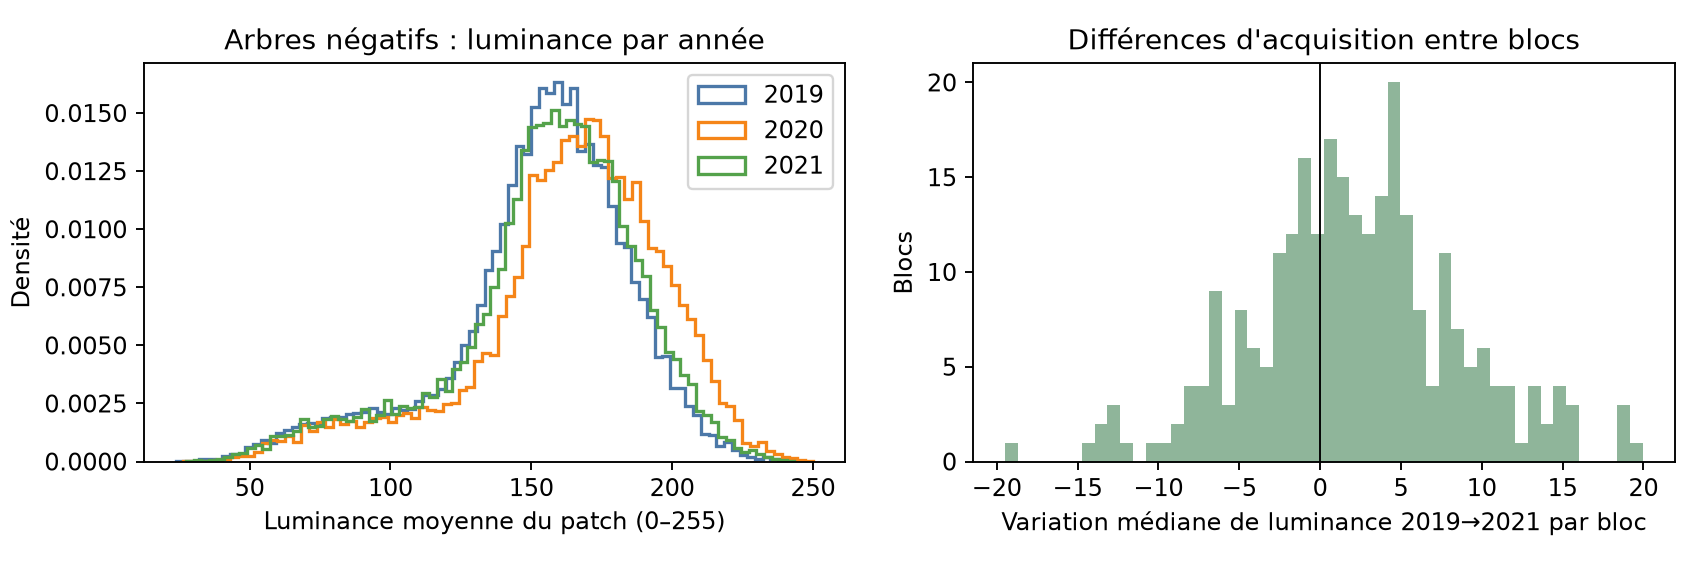
\includegraphics[width=\columnwidth]{figures/radiometrie.png}
\caption{Arbres négatifs : luminance par année (gauche) et variation médiane 2019$\to$2021 par bloc (droite).}
\label{fig:radio}
\end{figure}

% ============================= 3. MÉTHODES ================================
\section{Méthodes et protocole}
Les méthodes ne reçoivent pas la même information ; nous comparons des \emph{chaînes complètes}. \textbf{Seuil} : baisse
d'intensité entre dates. \textbf{CUSUM} : cumul des baisses au-delà d'une tolérance $k$. \textbf{Isolation Forest} : anomalie
sur les statistiques d'intensité. \textbf{TCN} : 4 statistiques $\times$ 3 dates. \textbf{Siamese CNN} : deux patches RGB (2019,
2021) encodés par un réseau à poids partagés (Table~\ref{tab:arch}). Normalisation et seuils sont ajustés sur l'entraînement et
la validation uniquement. Les grilles de la phase~1 sont petites (Table~\ref{tab:hp}) : 3 variantes par méthode, 6 pour CUSUM
qui croise deux paramètres ; le seuil maximise le F1 de validation.

\begin{table*}[t]
\centering\small
\caption{Phase 1 --- grilles explorées, configuration retenue en gras (sélection sur PR-AUC de validation).}
\label{tab:hp}
\setlength{\tabcolsep}{4pt}
\begin{tabular}{@{}lcL{11.2cm}r@{}}
\toprule
Méthode & Essais & Variantes explorées & PR-AUC val. \\
\midrule
Seuil & 3 & baisse totale ; \textbf{baisse annuelle maximale} ; baisse relative & 0,054 \\
CUSUM & 6 & absolu $k\in\{0;5;\mathbf{10}\}$ ; relatif $k\in\{0;0{,}03;0{,}06\}$ & 0,053 \\
Isolation Forest & 3 & (arbres, échantillons, variables) : (150, 256, 0,7) ; (250, 512, 1,0) ; \textbf{(350, 1024, 0,8)} & 0,030 \\
TCN & 3 & (lr, canaux, dropout, noyau) : \textbf{($10^{-3}$, 12, 0,10, 2)} ; ($4\cdot10^{-4}$, 20, 0,25, 2) ; ($7\cdot10^{-4}$, 16, 0,35, 3) ; 8 époques & 0,049 \\
Siamese CNN & 3 & (lr, largeur, dropout) : ($10^{-3}$, 8, 0,15) ; ($4\cdot10^{-4}$, 12, 0,25) ; \textbf{($7\cdot10^{-4}$, 16, 0,35)} ; 6 époques & 0,167 \\
\bottomrule
\end{tabular}
\end{table*}

\begin{table}[!htb]
\centering\footnotesize
\caption{Architectures (ReLU ; GAP : moyenne globale ; BN : normalisation par lots).}
\label{tab:arch}
\setlength{\tabcolsep}{2pt}
\begin{tabular}{@{}lL{1.3cm}L{3.4cm}r@{}}
\toprule
Modèle & Entrée & Corps et tête & Param. \\
\midrule
Siamese initial & $2{\times}3{\times}16^2$ & Conv(16)--Pool--Conv(32)--GAP ; $[|z_a{-}z_b|, z_a{\odot}z_b]\to32\to1$ & 7\,201 \\
Siamese v2 & $2{\times}3{\times}32^2$ & 3 blocs [Conv--BN--ReLU]$\times$2 (16, 32, 64) ; $[|z_a{-}z_b|, z_a{\odot}z_b, z_b{-}z_a]\to64\to1$, dropout 0,3 & 84\,721 \\
TCN & $4\times3$ & 2 blocs résiduels causaux, noyau 2, 12 canaux, dilatations 1 et 2 & 1\,081 \\
MLP (contrôle) & 12 & $12\to32\to1$ & 449 \\
\bottomrule
\end{tabular}
\end{table}

\textbf{Protocole en deux phases} (Figure~\ref{fig:proto}). En \textbf{phase~1}, tous les choix sont faits sur la validation et le
test est évalué une fois : ce sont les seuls résultats confirmatoires. La \textbf{phase~2} regroupe ce qui a été fait
\emph{après} consultation du test (Siamese~v2, graines, IC, fuite, validation croisée, ablation) : ces résultats sont
\textbf{rétrospectifs} et marqués \retro{}. Critère principal : PR-AUC (hasard = prévalence). IC95 par bootstrap des blocs
spatiaux (1\,000 tirages), comparaisons appariées sur les mêmes blocs.

\begin{figure}[!htb]
\centering
\begin{tikzpicture}[font=\scriptsize, node distance=2mm,
  b/.style={draw, rounded corners=2pt, align=center, minimum height=6mm, inner sep=2pt, fill=white},
  a/.style={-{Stealth[length=1.5mm]}}]
\node[b, fill=olive!12] (d) {OQDS\\71\,956 arbres};
\node[b, right=of d] (s) {Blocs 250\,m\\Train/Val/Test};
\node[b, right=of s, fill=olive!12] (v) {Sélection\\sur Val};
\node[b, below=3mm of v, fill=olive!25] (t) {\textbf{Test ouvert}\\\textbf{une fois} (ph. 1)};
\node[b, left=of t, fill=retro!15, text width=2.6cm] (r) {Phase 2 rétrospective : v2, IC, fuite, CV, ablation};
\node[b, left=of r, fill=gray!12, text width=1.2cm] (f) {Futur : région scellée};
\draw[a] (d) -- (s); \draw[a] (s) -- (v); \draw[a] (v) -- (t); \draw[a] (t) -- (r); \draw[a, dashed] (r) -- (f);
\end{tikzpicture}
\caption{Protocole : seule la phase 1 est confirmatoire.}
\label{fig:proto}
\end{figure}

% ======================= 4. RÉSULTATS PHASE 1 =============================
\section{Résultats pré-spécifiés (phase 1)}
La Table~\ref{tab:main} sépare les mesures indépendantes du seuil (ROC-AUC, PR-AUC) des mesures au seuil fixé sur validation,
puis les traduit en alertes.

\begin{table*}[t]
\centering\small
\caption{Phase 1 --- test (10\,205 arbres, 237 positifs). Seuils fixés sur validation ; IC95 par blocs spatiaux. « Alertes/VP » :
arbres à inspecter par disparition réelle trouvée.}
\label{tab:main}
\setlength{\tabcolsep}{3.6pt}
\begin{tabular}{@{}l ccc ccc rrr r@{}}
\toprule
& \multicolumn{3}{c}{Indépendant du seuil} & \multicolumn{3}{c}{Au seuil} & \multicolumn{4}{c}{Charge d'alerte} \\
\cmidrule(lr){2-4}\cmidrule(lr){5-7}\cmidrule(lr){8-11}
Méthode & ROC-AUC & PR-AUC & IC95 PR-AUC & Préc. & Rappel & F1 & VP & FP & FN & Alertes/VP \\
\midrule
\textbf{Siamese CNN} & \textbf{0,874} & \textbf{0,220} & [0,032 ; 0,442] & \textbf{0,301} & 0,346 & \textbf{0,322} & 82 & 190 & 155 & \textbf{3,3} \\
TCN & 0,763 & 0,062 & [0,007 ; 0,147] & 0,055 & \textbf{0,692} & 0,103 & 164 & 2\,795 & 73 & 18,0 \\
CUSUM & 0,652 & 0,039 & [0,006 ; 0,090] & 0,047 & 0,143 & 0,071 & 34 & 684 & 203 & 21,1 \\
Seuil & 0,625 & 0,033 & [0,005 ; 0,078] & 0,032 & 0,068 & 0,044 & 16 & 478 & 221 & 30,9 \\
Isolation Forest & 0,556 & 0,026 & [0,004 ; 0,057] & 0,027 & \textbf{0,692} & 0,051 & 164 & 5\,975 & 73 & 37,4 \\
\bottomrule
\end{tabular}
\end{table*}

\textbf{Siamese CNN.} Parmi les cinq chaînes, il a la meilleure PR-AUC, la meilleure ROC-AUC et le meilleur F1 ; son avantage
de PR-AUC est significatif face à chaque méthode (bootstrap apparié : $+0{,}15$ [0,02~;~0,31] sur le TCN, $+0{,}18$ à $+0{,}19$
sur les autres). Mais au seuil retenu, il déclenche 272 alertes (82 justes, 190 fausses) et manque 155 positifs : ce n'est pas
un détecteur utilisable sans contrôle humain. Il ne domine pas toutes les métriques : le TCN et Isolation Forest ont un
meilleur rappel (0,692), au prix de 18 à 37 inspections par cas réel.

\textbf{Pourquoi le TCN fait tant de fausses alertes.}\label{sec:fp} Parmi les négatifs, son score est corrélé à la baisse
d'intensité ($r=-0{,}72$) et 99,5\,\% de ses fausses alertes concernent des arbres dont l'intensité baisse. Dans le quart des
blocs où la baisse est la plus forte, il signale à tort 41\,\% des arbres (16\,\% dans le quart le moins touché), contre 5\,\%
pour le Siamese~v2\retro{} (Table~\ref{tab:fp}). Il confond un changement d'acquisition avec une disparition ; une normalisation
locale de l'intensité par bloc serait nécessaire.

\begin{table}[!htb]
\centering\footnotesize
\caption{Fausses alertes sur les négatifs du test, par quartile de variation d'intensité de leur bloc (2019$\to$2021).}
\label{tab:fp}
\setlength{\tabcolsep}{3pt}
\begin{tabular}{@{}lrrr@{}}
\toprule
Quartile (variation médiane) & Négatifs & FP TCN & FP v2\retro{} \\
\midrule
Q1 : baisse forte ($-52$) & 2\,573 & 41,3\,\% & 5,4\,\% \\
Q2 ($-47$) & 2\,511 & 29,7\,\% & 1,8\,\% \\
Q3 ($-42$) & 2\,493 & 24,0\,\% & 3,5\,\% \\
Q4 : baisse faible ($-31$) & 2\,391 & 16,2\,\% & 1,3\,\% \\
\bottomrule
\end{tabular}
\end{table}

% ======================= 5. ANALYSES RÉTROSPECTIVES ========================
\section{Analyses rétrospectives (phase 2)}
\subsection{Siamese v2, variabilité et seuils}
Réentraînées avec 5 graines, les configurations de phase~1 donnent $0{,}215\pm0{,}039$ (Siamese) et $0{,}058\pm0{,}004$ (TCN) :
le classement ne dépend pas d'une graine. Avec 6 époques, le Siamese était sous-entraîné (0,167 en validation, 0,228 en
entraînant plus longtemps). Parmi quatre configurations comparées \emph{sur la validation}, la meilleure (Siamese~v2) utilise des
patches de 32$\times$32 pixels (16\,m ; 0,293 contre 0,265 en 16$\times$16 : le contexte aide), la normalisation par lots,
une augmentation identique aux deux dates, AdamW, une pondération $\sqrt{n_-/n_+}$ et un arrêt anticipé (patience 7, au plus 40
époques). La PR-AUC d'entraînement monte jusqu'à 0,6--0,7 alors que celle de validation plafonne : l'arrêt anticipé limite ce
surapprentissage, et les scores de 5 graines sont moyennés (Figure~\ref{fig:lc}).

\begin{figure*}[t]
\centering
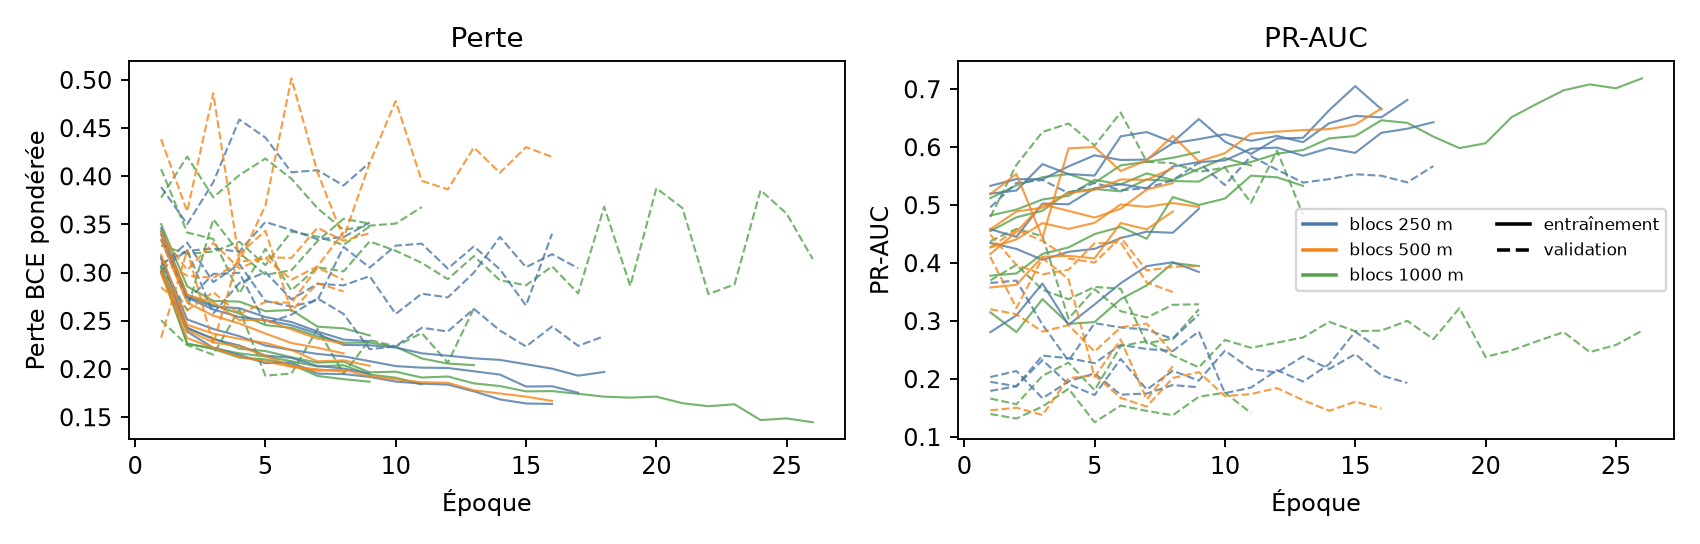
\includegraphics[width=0.78\textwidth]{figures/curves_cv.png}
\caption{Courbes d'apprentissage\retro{} des 15 modèles v2 de la validation croisée (traits pleins : entraînement ; pointillés :
validation). La PR-AUC d'entraînement monte alors que celle de validation plafonne : l'arrêt anticipé limite le surapprentissage.}
\label{fig:lc}
\end{figure*}

\begin{table}[!htb]
\centering\footnotesize
\caption{Siamese v2\retro{} et budgets d'inspection (test ; seuils fixés sur validation).}
\label{tab:v2}
\setlength{\tabcolsep}{1.2pt}
\begin{tabular}{@{}lcc@{}}
\toprule
& Siamese initial & Siamese v2\retro{} \\
\midrule
PR-AUC validation & 0,167 & 0,314 \\
PR-AUC test (5 gr.) & $0{,}215\pm0{,}039$ & $0{,}468\pm0{,}050$ \\
PR-AUC test, ens. [IC95] & 0,22 [0,03;0,44] & 0,49 [0,11;0,73] \\
ROC-AUC test & 0,874 & 0,961 \\
Préc. / rappel / F1 & 0,30 / 0,35 / 0,32 & 0,36 / 0,72 / 0,48 \\
VP / FP / FN & 82 / 190 / 155 & 171 / 302 / 66 \\
\midrule
Budget 2\,\% : rappel/préc. & 26 / 34\,\% & 55 / 50\,\% \\
Budget 5\,\% : rappel/préc. & 47 / 25\,\% & 76 / 31\,\% \\
À inspecter pour rappel $\geq$80\,\% & 30,8\,\% & 13,4\,\% \\
\bottomrule
\end{tabular}
\end{table}

\begin{figure}[!htb]
\centering
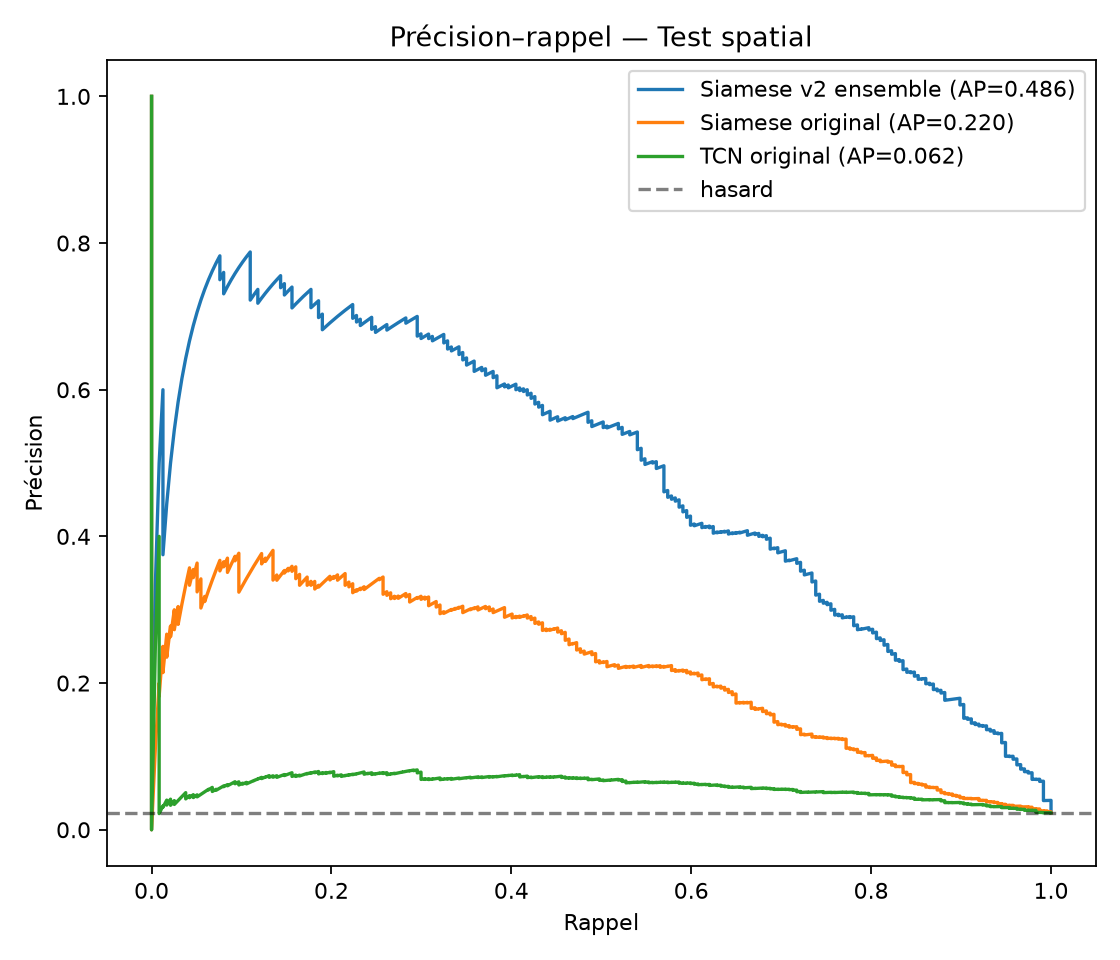
\includegraphics[width=0.92\columnwidth]{figures/pr_curves_original_vs_improved.png}
\caption{Courbes précision--rappel sur le test : Siamese v2\retro{} (ensemble), Siamese initial et TCN. Pointillés : prévalence.}
\label{fig:pr}
\end{figure}

Le v2 retrouve 171 positifs au lieu de 82 (Table~\ref{tab:v2}, Figure~\ref{fig:pr}) ; le gain apparié est de $+0{,}24$ [0,08~;~0,35]. Le seuil doit
suivre la capacité d'inspection : en inspectant 2\,\% des arbres, le v2 retrouve plus de la moitié des disparitions, avec une
alerte juste sur deux ; pour 80\,\% de rappel, il faut inspecter 13\,\% des arbres (31\,\% avec le Siamese initial, 55\,\% avec
le TCN). L'IC95 reste large, car tous les positifs du test sont dans 5 blocs.

\subsection{Fuite spatiale et validation croisée}
\label{sec:leak}
\textbf{Fuite.} En retirant du test les arbres proches d'un arbre d'entraînement (Table~\ref{tab:leak}), la ROC-AUC du v2 reste
stable et la PR-AUC reste 21 à 24 fois la prévalence jusqu'à 50\,m ; à 100\,m, il ne reste que 13 positifs. Un modèle qui ne
voit que 2019 reste au niveau du hasard (0,039) : pas de raccourci contextuel.

\begin{table}[!htb]
\centering\footnotesize
\caption{Siamese v2\retro{} : test restreint aux arbres à plus de $d$ m de tout arbre d'entraînement.}
\label{tab:leak}
\setlength{\tabcolsep}{3.5pt}
\begin{tabular}{@{}rrrrrr@{}}
\toprule
$d$ (m) & Arbres & Pos. & ROC-AUC & PR-AUC & PR/prév. \\
\midrule
0 & 10\,205 & 237 & 0,961 & 0,486 & 20,9 \\
16 & 8\,989 & 178 & 0,963 & 0,426 & 21,5 \\
32 & 7\,537 & 108 & 0,965 & 0,339 & 23,7 \\
50 & 6\,065 & 61 & 0,955 & 0,234 & 23,3 \\
100 & 2\,760 & 13 & 0,877 & 0,026 & 5,5 \\
\bottomrule
\end{tabular}
\end{table}

\textbf{Validation croisée spatiale.} Pour tester d'autres zones, nous refaisons le découpage avec des blocs de 250\,m, 500\,m et
1\,km, en 5 partitions chacun (test $k$, validation $k+1$, entraînement sur le reste), soit 15 modèles v2 (Table~\ref{tab:cv}).

\begin{table}[!htb]
\centering\footnotesize
\caption{Validation croisée spatiale\retro{} (un modèle v2 par partition) : moyenne $\pm$ écart-type et [min ; max].}
\label{tab:cv}
\setlength{\tabcolsep}{2.5pt}
\begin{tabular}{@{}lccc@{}}
\toprule
& 250\,m & 500\,m & 1\,km \\
\midrule
Blocs test avec positifs & 10,2 & 7,2 & 4,4 \\
PR-AUC test & $0{,}33\pm0{,}14$ & $0{,}32\pm0{,}13$ & $0{,}33\pm0{,}19$ \\
\quad [min ; max] & [0,19 ; 0,52] & [0,17 ; 0,53] & [0,14 ; 0,55] \\
ROC-AUC test & $0{,}92\pm0{,}03$ & $0{,}91\pm0{,}03$ & $0{,}91\pm0{,}04$ \\
F1 test & $0{,}35\pm0{,}11$ & $0{,}36\pm0{,}11$ & $0{,}36\pm0{,}15$ \\
\bottomrule
\end{tabular}
\end{table}

(1) \textbf{La taille des blocs ne change pas la moyenne} : éloigner davantage entraînement et test ne fait pas chuter le
modèle, ce qui confirme l'absence de fuite importante. (2) \textbf{La performance dépend de la zone} (0,14 à 0,55). (3) \textbf{Le
test d'origine est favorable} : un v2 seul y obtient 0,42--0,53, contre 0,33 en moyenne ici. L'estimation prudente pour une zone
nouvelle du même secteur est donc d'environ \textbf{0,33} (11 fois le hasard). Toutes ces zones appartiennent au même secteur
de 35\,km$^2$ : la généralisation à d'autres régions (par exemple des oliveraies marocaines) n'est pas testée.

\subsection{Ablation, déséquilibre et attention}
\label{sec:abl}
Chaque variante est entraînée avec les mêmes hyperparamètres et trois graines (Table~\ref{tab:abl}). Avec 2019 seule, le modèle
est au niveau du hasard ; avec 2021 seule, il perd 0,12 à 0,15 : c'est la \emph{comparaison} des deux dates qui porte le signal,
ce qui répond à RQ1. Le partage des poids donne le même score avec deux fois moins de paramètres. Sans couleur, la validation
baisse de 0,06. Ajouter 2020 est la meilleure variante. Pour le déséquilibre, la pondération $\sqrt{n_-/n_+}$ reste la meilleure ;
la perte focale fait jeu égal (0,292 contre 0,293 en validation) et le rééchantillonnage, simple ou spatial, favorise le
surapprentissage. L'attention apporte un léger gain, dans la variabilité entre zones. Enfin, un MLP sur les 12 valeurs du TCN
fait aussi bien que lui ($0{,}052$ contre $0{,}058$) : sur 3 dates, la convolution temporelle n'apporte rien.

\begin{table}[!htb]
\centering\footnotesize
\caption{Ablation et variantes\retro{} du Siamese v2 : PR-AUC moyenne $\pm$ écart-type (3 graines).}
\label{tab:abl}
\setlength{\tabcolsep}{2.5pt}
\begin{tabular}{@{}lrcc@{}}
\toprule
Variante & Param. & Validation & Test \\
\midrule
Référence (2019+2021) & 84\,721 & 0,297 $\pm$ 0,011 & 0,434 $\pm$ 0,017 \\
3 dates (2019--2021) & 88\,817 & \textbf{0,368 $\pm$ 0,031} & 0,484 $\pm$ 0,053 \\
Sans partage des poids & 157\,025 & 0,297 $\pm$ 0,017 & 0,454 $\pm$ 0,085 \\
Niveaux de gris & 84\,433 & 0,235 $\pm$ 0,013 & 0,446 $\pm$ 0,081 \\
2021 seule & 76\,529 & 0,175 $\pm$ 0,013 & 0,283 $\pm$ 0,043 \\
2019 seule (contrôle) & 76\,529 & 0,037 $\pm$ 0,004 & 0,039 $\pm$ 0,005 \\
\midrule
Attention (SE) & 87\,614 & 0,306 $\pm$ 0,017 & \textbf{0,490 $\pm$ 0,019} \\
Rééch. équilibré & 84\,721 & 0,284 $\pm$ 0,028 & 0,358 $\pm$ 0,048 \\
Rééch. spatial & 84\,721 & 0,212 $\pm$ 0,031 & 0,364 $\pm$ 0,117 \\
\bottomrule
\end{tabular}
\end{table}

\subsection{Robustesse et exemples}
\label{sec:robust}
\textbf{Pixels noirs.} Sur les 80,7\,\% de patches test sans pixel noir, le Siamese initial obtient F1 = 0,333 ; neutraliser les
pixels transparents (34 arbres) ne change aucune décision. \textbf{Éclairage.} Avec des perturbations synthétiques appliquées à
tous les patches test (Table~\ref{tab:robust}), le v2 résiste à un assombrissement, à une zone masquée et à un gamma, mais
\textbf{se dégrade} fortement si 2021 est éclaircie, perd du contraste ou reçoit une ombre portée ; le nombre d'alertes au seuil
fixe varie alors de 1 à 1\,067. L'augmentation utilisée ($\pm$10\,\%) est trop faible : une normalisation radiométrique entre
dates est nécessaire.

\begin{table}[!htb]
\centering\footnotesize
\caption{Robustesse\retro{} du v2 à des perturbations synthétiques (seuil fixe 0,72).}
\label{tab:robust}
\setlength{\tabcolsep}{3pt}
\begin{tabular}{@{}lrr@{}}
\toprule
Perturbation & PR-AUC & Alertes \\
\midrule
Aucune (référence) & 0,486 & 473 \\
2021 assombrie ($\times$0,8) & 0,482 & 118 \\
Zone masquée 10$\times$10 px sur 2021 & 0,460 & 374 \\
Gamma 1,25 sur 2021 & 0,545 & 248 \\
Bord noir de 6 px sur 2021 & 0,394 & 135 \\
Ombre portée sur 2019 & 0,401 & 662 \\
Contraste 2021 $\times$0,7 & 0,284 & 845 \\
2021 éclaircie ($\times$1,2) & 0,278 & 1\,067 \\
Ombre portée sur 2021 & 0,237 & 1 \\
\bottomrule
\end{tabular}
\end{table}

\textbf{Exemples} (Figure~\ref{fig:ex}). Le vrai positif montre une couronne nette en 2019--2020 puis absente en 2021 ; le faux
positif, un fort changement d'éclairage sans disparition ; le faux négatif est en bord de raster. OQDS n'a pas de classe
« dépérissant » : un arbre affaibli mais présent est négatif, et aucune image ne confirme l'état sanitaire réel.

\begin{figure}[!htb]
\centering
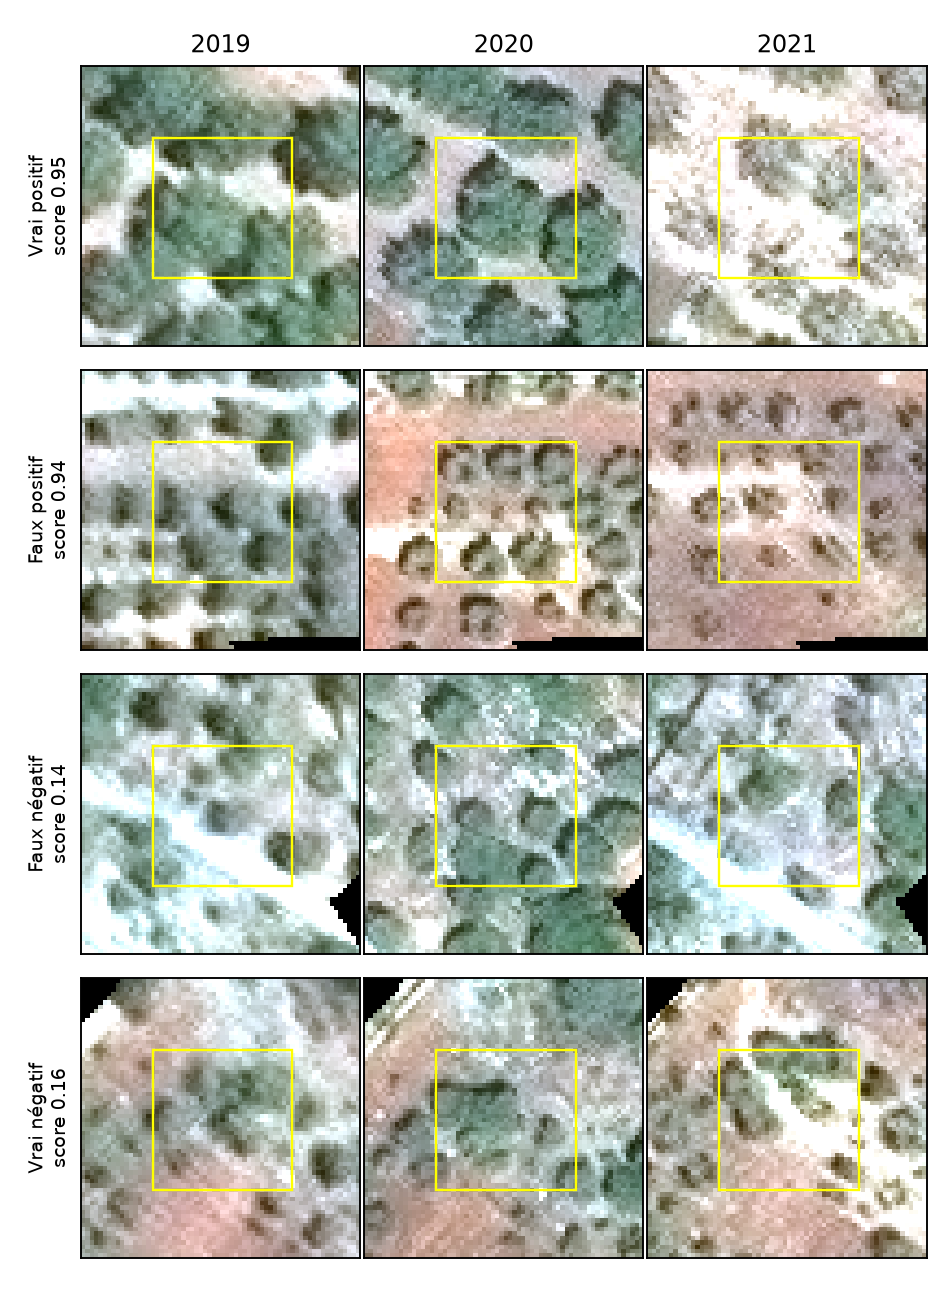
\includegraphics[width=0.66\columnwidth]{figures/examples_confusion_compact.png}
\caption{Exemples\retro{} réels du v2 au seuil 0,72 (6\textsuperscript{e} cas le plus extrême de chaque catégorie, vrai négatif
tiré au hasard ; arbres OQDS 56610, 73872, 36678, 19267). « Positif » = disparition apparente, sans preuve de maladie.}
\label{fig:ex}
\end{figure}

% ============================ 6. DISCUSSION ===============================
\section{Discussion}
\textbf{Réponses.} RQ1 : oui, dans ce corpus, et l'ablation attribue le gain à la comparaison d'images. RQ2 : le Siamese offre
le meilleur compromis (3,3 alertes par cas réel en phase~1, 13\,\% d'arbres à inspecter pour 80\,\% de rappel avec le v2). RQ3 :
pas de dépendance aux pixels noirs, mais une sensibilité réelle à l'éclairage.

\textbf{Validité et limites.} (i) La cible est indirecte. (ii) Les observations sont groupées : la validation croisée couvre
d'autres zones, mais du même secteur. (iii) Les exclusions introduisent un léger biais. (iv) Le test principal a déjà été
consulté. (v) La recherche d'hyperparamètres reste restreinte (CPU) ; les U-Net et Transformers de détection de changement
n'ont pas été testés, car ils demandent des masques par pixel ou de longues séries absents du corpus. (vi) L'étude par type
de changement (couronne réduite, végétation voisine, etc.) demande des annotations qu'OQDS ne fournit pas. L'expérience
hyperspectrale (ROC-AUC 0,798, 76 arbres) reste exploratoire ; NEON et CrownsDb ne peuvent pas servir de test externe.

\textbf{Modèle retenu.} Le Siamese~v2 est choisi sur la validation (0,314 contre 0,167 pour le Siamese initial et 0,054 au mieux
pour les autres méthodes) ; la variante à trois dates est la prochaine évolution. Ces choix restent à confirmer sur un test
nouveau.

\textbf{Intégration (conception).} Un microservice \textbf{FastAPI} chargera une fois l'ensemble v2, sa normalisation et son seuil,
et sera appelé par \textbf{Spring Boot} via \texttt{GET /health}, \texttt{GET /model}, \texttt{POST /predict} (un arbre :
coordonnées et deux patches en base64) et \texttt{POST /predict/batch} (asynchrone, références de rasters). La réponse contient
\texttt{tree\_id}, \texttt{x}, \texttt{y}, \texttt{crs}, \texttt{dates}, \texttt{score}, \texttt{threshold},
\texttt{predicted\_class} (« disparition\_apparente » ou non, jamais « malade »), \texttt{model\_version} (empreinte du
checkpoint) et des \texttt{warnings} (pixels noirs, écart radiométrique), par exemple :\par
{\footnotesize
\begin{verbatim}
{"tree_id":"26925","x":708258.5,"y":4513499.8,
 "crs":"EPSG:32633","dates":["2019","2021"],
 "score":0.83,"threshold":0.72,
 "predicted_class":"disparition_apparente",
 "model_version":"siamese_v2_ens5@3f9a1c2e",
 "warnings":["pixels_noirs_2021 > 20 %"]}
\end{verbatim}
}
\noindent La Table~\ref{tab:bench} compare les coûts sur un même CPU ; aucune latence de service HTTP n'a encore été mesurée.

\begin{table}[!htb]
\centering\footnotesize
\caption{Coût de calcul sur un même CPU (32 threads logiques, PyTorch 2.15) : latence d'un arbre (1 thread, médiane de 300
appels) et durée pour les 10\,205 arbres test (8 threads), patches déjà extraits.}
\label{tab:bench}
\setlength{\tabcolsep}{2.5pt}
\begin{tabular}{@{}lrrrr@{}}
\toprule
Méthode & Param. & Poids & 1 arbre & 10\,205 arbres \\
\midrule
Seuil / CUSUM & 1--2 & $<$1\,ko & 0,05--0,44\,ms & $<$1\,ms \\
TCN & 1\,081 & 9\,ko & 0,41\,ms & 8\,ms \\
Isolation Forest & 113\,890\textsuperscript{*} & 9,7\,Mo & 36,6\,ms & 0,37\,s \\
Siamese initial & 7\,201 & 32\,ko & 0,47\,ms & 0,21\,s \\
Siamese v2 & 84\,721 & 0,34\,Mo & 2,7\,ms & 2,9\,s \\
Siamese v2 (ens. 5) & 423\,605 & 1,7\,Mo & 14,7\,ms & 14,8\,s \\
\bottomrule
\multicolumn{5}{@{}l}{\textsuperscript{*} nombre de nœuds des arbres}
\end{tabular}
\end{table}

\textbf{Reproductibilité.} Code, configurations gelées, checkpoints, prédictions et historiques sont versionnés dans le dépôt
\texttt{Project-JEE-DL} (Python 3.12, PyTorch 2.15 CPU, graine 20261106). Le rechargement de l'ensemble reproduit ses scores à
$10^{-7}$ près ; la chaîne complète reste à réexécuter dans un environnement isolé.

% =========================== 7. FUTUR PROTOCOLE ===========================
\section{Protocole de validation futur}
\label{sec:future}
Le prochain test sera fixé \emph{avant} expérimentation : (1) une région ou exploitation indépendante, scellée jusqu'au gel du
modèle et du seuil ; (2) une zone tampon d'au moins 50\,m~\cite{valavi} ; (3) un critère unique (PR-AUC), des budgets
d'inspection de 2 et 5\,\%, 5 graines et des IC par blocs ; (4) des règles d'exclusion écrites à l'avance ; (5) une vérification
terrain de toutes les alertes d'un budget de 2\,\% et d'un tirage de non-alertes, avec la cause (arraché, mort sur pied,
dépérissant, couronne réduite, différence d'acquisition) ; (6) idéalement, un proxy infrarouge calibré pour détecter le
dépérissement. Le test actuel reste réservé au diagnostic rétrospectif.

% ============================ 8. CONCLUSION ===============================
\section{Conclusion}
Dans la phase pré-spécifiée, le Siamese CNN est le meilleur des cinq pipelines (PR-AUC 0,220, F1 0,322) mais ne retrouve que 82
des 237 positifs. Après correction de son sous-entraînement, le Siamese~v2 atteint 0,486 sur le test d'origine et environ 0,33 en
moyenne sur 15 partitions géographiques, soit 11 fois le hasard ; l'ablation attribue ce gain à la comparaison des deux dates.
Trois problèmes doivent rester séparés : \textbf{détecter la disparition} d'une couronne, ce que mesure ce travail ;
\textbf{identifier le dépérissement} d'un arbre encore présent, qui exige une étiquette graduée et un proxy infrarouge ;
\textbf{diagnostiquer une maladie}, qui exige une vérité biologique de terrain. Nos résultats ne portent que sur le premier :
ils justifient un outil de priorisation des inspections, pas un diagnostic automatique.

{\footnotesize
\begin{thebibliography}{99}
\setlength{\itemsep}{0pt}
\bibitem{oqds} Crecco et al., article de données OQDS, \emph{Data in Brief}, 2025. doi:10.1016/j.dib.2025.111615.
\bibitem{lin} Lin et al., cartographie d'oliviers, \emph{ISPRS J. Photogramm. Remote Sens.}, 2024. doi:10.1016/j.isprsjprs.2024.08.003.
\bibitem{raouhi} E. M. Raouhi et al., « Optimization techniques in deep convolutional neuronal networks applied to olive diseases classification », \emph{Artif. Intell. Agric.}, 6:77--89, 2022.
\bibitem{bromley} J. Bromley et al., « Signature verification using a Siamese time delay neural network », \emph{NeurIPS}, 1993.
\bibitem{daudt} R. C. Daudt, B. Le Saux, A. Boulch, « Fully convolutional Siamese networks for change detection », \emph{IEEE ICIP}, 2018.
\bibitem{page} E. S. Page, « Continuous inspection schemes », \emph{Biometrika}, 41:100--115, 1954.
\bibitem{iforest} F. T. Liu, K. M. Ting, Z.-H. Zhou, « Isolation Forest », \emph{IEEE ICDM}, 2008.
\bibitem{bai} S. Bai, J. Z. Kolter, V. Koltun, « An empirical evaluation of generic convolutional and recurrent networks for sequence modeling », arXiv:1803.01271, 2018.
\bibitem{roberts} D. R. Roberts et al., « Cross-validation strategies for data with temporal, spatial, hierarchical, or phylogenetic structure », \emph{Ecography}, 40:913--929, 2017.
\bibitem{valavi} R. Valavi et al., « blockCV: An R package for generating spatially or environmentally separated folds for k-fold cross-validation of species distribution models », \emph{Methods Ecol. Evol.}, 10(2):225--232, 2019.
\bibitem{saito} T. Saito, M. Rehmsmeier, « The precision-recall plot is more informative than the ROC plot when evaluating binary classifiers on imbalanced datasets », \emph{PLoS ONE}, 10(3), 2015.
\bibitem{neon} weecology, « NEON tree crowns », Hugging Face Datasets.
\bibitem{hyper} « Olive hyperspectral stress », Zenodo, record 10336545.
\bibitem{crowns} Y. Hnida et al., « OliveTreeCrownsDb », Mendeley Data, v2, 2024.
\end{thebibliography}
}

\end{document}
